\subsection{Blob Detection}
\label{sec:blob-detection}

\subsubsection{Apply blob detection to the dataset}
A multiscale Laplacian-of-Gaussian (LoG) detector was applied to all 1,310
images to locate bright and dark regions and estimate their spatial scale.
Images were EXIF-oriented, resized to a maximum side of 512 pixels without
enlargement, and converted to grayscale intensities in $[0,1]$. Aspect ratios
were preserved; all subsequent measurements refer to processed-image pixels.

The detector smooths the image and measures local intensity curvature at
several scales. For grayscale image $I$, this gives the response
\begin{equation}
 \boxed{R_\sigma(x,y)=-\sigma^2\nabla^2(G_\sigma*I)(x,y)}.
 \label{eq:blob-log}
\end{equation}
In Equation~\eqref{eq:blob-log}, $(x,y)$ is pixel position, $G_\sigma$ is a
Gaussian filter with standard deviation $\sigma$, and $*$ denotes convolution.
The Laplacian $\nabla^2$ sums the second spatial derivatives. Small values of
$\sigma$ examine fine structures; larger values examine broader regions.
Multiplication by $\sigma^2$ normalizes the response across scales, while the
minus sign assigns positive responses to bright centers and negative responses
to dark centers.

Candidate centers are local maxima of the absolute response within three rows,
three columns, and three neighboring scale levels. A response threshold
$\tau$ excludes weak candidates. Each remaining candidate receives radius
$r=\sqrt{2}\sigma$, an estimate of feature scale rather than an object boundary.
Circles crossing the frame are excluded. Candidates are then processed
strongest first, discarding those whose overlap with a retained circle exceeds
a specified fraction of the smaller circle's area.

These decisions require a common configuration before results can be compared.
Table~\ref{tab:blob-baseline-settings} defines that reference configuration,
called the baseline, and the role of each parameter. The values were selected
through visual inspection of the display examples described below, rather than
optimization against annotated data. Additional pre-smoothing is disabled
because Gaussian smoothing is already part of LoG; its effect is tested later.

\begin{table}[H]
\centering
\small
\caption{Blob-detector parameters and baseline values. Scale and smoothing
values are measured in processed-image pixels.}
\label{tab:blob-baseline-settings}
\begin{tabular}{@{}p{0.24\linewidth}p{0.14\linewidth}p{0.54\linewidth}@{}}
\toprule
Parameter & Baseline & Function \\
\midrule
Minimum scale, $\sigma_{\min}$ & 4 & Smallest Gaussian scale examined; sets the lower feature-size limit. \\
Maximum scale, $\sigma_{\max}$ & 16 & Largest Gaussian scale examined; sets the upper feature-size limit. \\
Number of scales & 12 & Number of filter scales between the limits, spaced with a constant ratio. \\
Response threshold, $\tau$ & 0.15 & Minimum absolute LoG response required for a candidate. \\
Overlap limit & 0.5 & Maximum permitted intersection as a fraction of the smaller circle's area. \\
Pre-smoothing, $\sigma_{\mathrm{pre}}$ & 0 & Gaussian smoothing before LoG filtering; zero disables this additional step. \\
\bottomrule
\end{tabular}
\end{table}

SciPy supplies the Gaussian derivatives and neighborhood maxima; candidate
selection and suppression are implemented explicitly. Synthetic checks verified
centers, polarity, approximate scales, and no detections on a constant image.

\subsubsection{Visualize the detected blobs}
All images were processed and received numbered overlays. For presentation,
ten fixed examples were selected by sorting filenames alphabetically within
each vehicle class and taking the first two from each of the five classes.
This provides reproducible examples from every class without reproducing all
1,310 outputs. It is not a random or representative sample, and it does not
limit the full-dataset blob calculations.

Figure~\ref{fig:blob-example} shows two of these examples: a pickup with repeated
trim features and a sedan with broader window and body regions. They were
selected to examine how local structure affects the detections. Yellow circles
mark bright responses and cyan circles dark responses.

\begin{figure}[H]
 \centering
 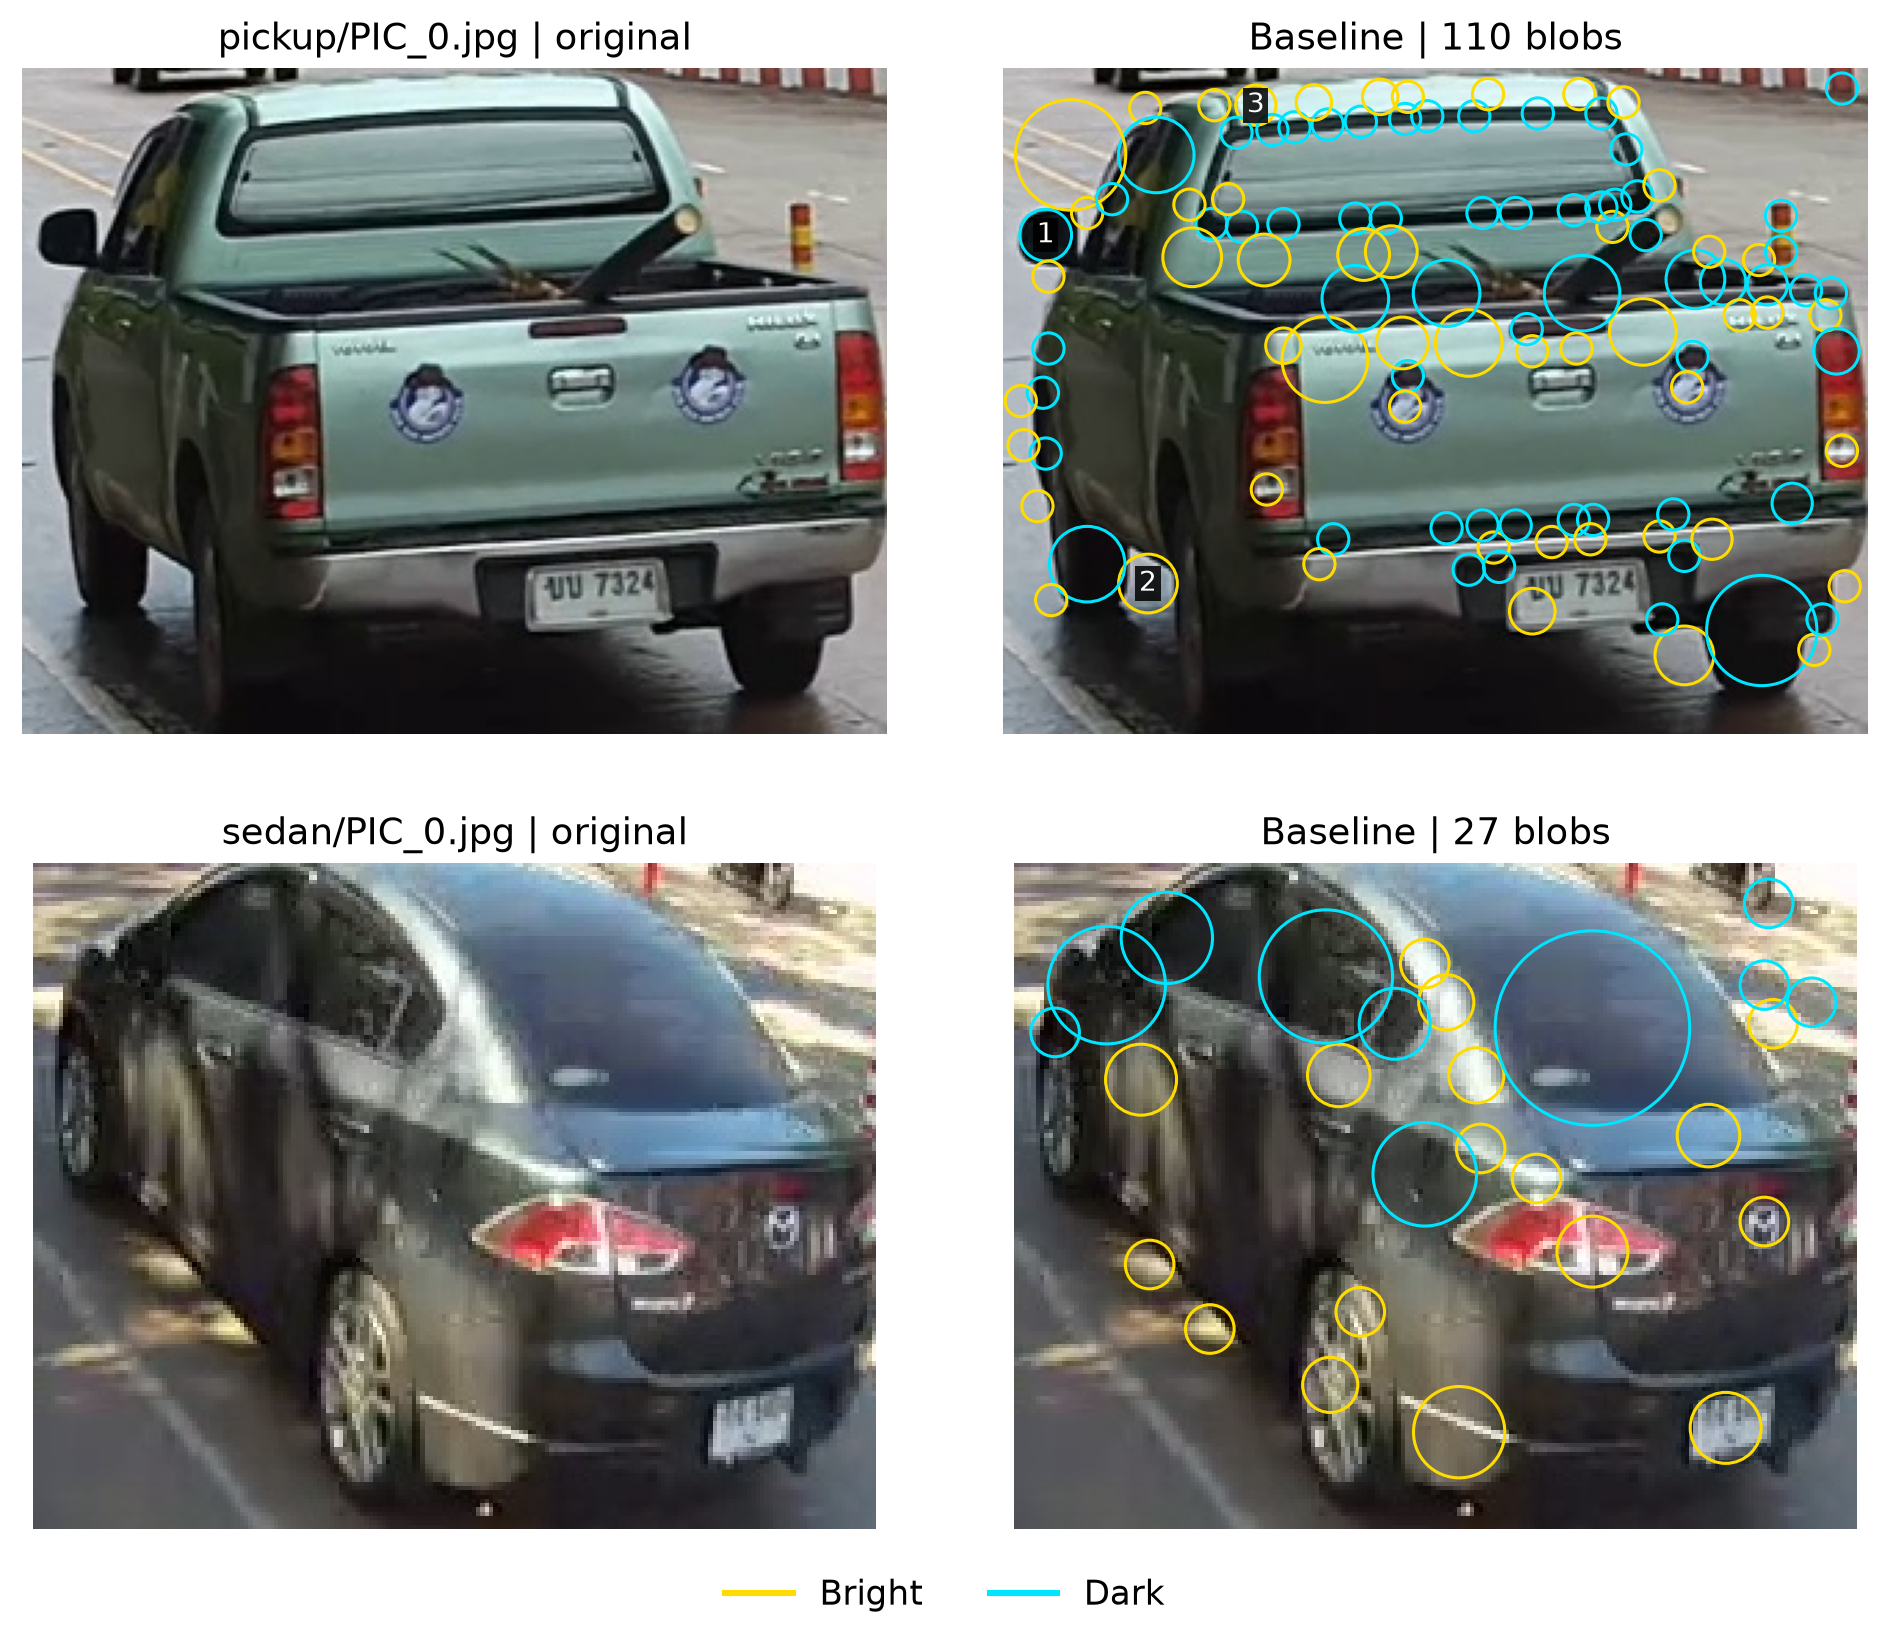
\includegraphics[width=0.92\linewidth]{Images/blob_report_baseline.png}
 \caption{Originals and baseline detections for two display examples, at
 processed resolution. Yellow circles mark bright blobs and cyan circles dark
 blobs. Only pickup IDs 1--3 are printed for readability;
 every detected circle is shown.}
 \label{fig:blob-example}
\end{figure}

The pickup has repeated responses along the window edges and bumper. The
sedan has a large dark response on part of its rear window, alongside smaller
responses on reflections and other details. Background regions are marked in
both images. The output therefore describes local contrast, not vehicle
instances or complete object outlines.

\subsubsection{Calculate and display counts, sizes, and positions}
Across the full dataset, the baseline produced 85,074 blobs with a mean radius
of 7.40 pixels. Counts range from 3 to 209 per image; the median is 63, and the
middle 50\% of images have 42--83 detections. Thus, the total combines images
with substantially different numbers of local responses.

Table~\ref{tab:blob-image-stats} reports counts and mean radii for the ten fixed
display examples. These are excerpts from the complete per-image results.

\begin{table}[htbp]
\centering
\small
\caption{Blob baseline for the ten display images. Mean radius is measured in processed-image pixels. Full statistics cover all 1,310 images.}
\label{tab:blob-image-stats}
\begin{tabular}{lrr}
\toprule
Image & Blobs & Mean radius (px) \\
\midrule
hatchback/PIC\_0.jpg & 33 & 7.22 \\
hatchback/PIC\_1.jpg & 85 & 7.70 \\
motorcycle/PIC\_0.jpg & 83 & 7.23 \\
motorcycle/PIC\_10.jpg & 19 & 6.10 \\
pickup/PIC\_0.jpg & 110 & 6.96 \\
pickup/PIC\_1.jpg & 106 & 6.74 \\
sedan/PIC\_0.jpg & 27 & 8.14 \\
sedan/PIC\_1.jpg & 70 & 9.68 \\
suv/PIC\_0.jpg & 107 & 7.12 \\
suv/PIC\_1.jpg & 55 & 8.21 \\
\bottomrule
\end{tabular}
\end{table}

To connect these summaries to individual detections,
Table~\ref{tab:blob-positions} gives the first three pickup blobs, whose IDs
are marked in the overlay. Coordinates begin at the top-left corner, with $x$
increasing rightward and $y$ downward. Radius $r$ determines the plotted circle;
its diameter and approximate area are $2r$ and $\pi r^2$. These are image-feature
measurements, not physical vehicle dimensions.

\begin{table}[htbp]
\centering
\small
\caption{First three numbered blobs in \texttt{pickup/PIC\_0.jpg}. Coordinates and estimated radii are in processed-image pixels; all detections are retained in the CSV export.}
\label{tab:blob-positions}
\begin{tabular}{rrrrl}
\toprule
ID & $x$ & $y$ & $r$ & Polarity \\
\midrule
1 & 15 & 60 & 9.36 & dark \\
2 & 52 & 186 & 10.62 & bright \\
3 & 91 & 13 & 7.28 & bright \\
\bottomrule
\end{tabular}
\end{table}

CSV exports retain all 1,310 image summaries and 85,074 individual blob records.
The measurements describe where the detector responds and at what scale.
Without annotated blobs, they do not establish detection accuracy.

\subsubsection{Evaluate the effect of algorithm parameters}
The baseline results depend on which scales and response strengths are
retained. To distinguish these effects, six variants were evaluated on all
1,310 images, each changing one baseline parameter. Table~\ref{tab:blob-parameters}
summarizes their counts and blob-weighted mean radii.

\begin{table}[htbp]
\centering
\small
\caption{Blob parameter experiments on all 1,310 images. Each variant changes only the specified parameter from baseline. Mean radius is weighted over individual blobs, in processed pixels.}
\label{tab:blob-parameters}
\begin{tabular}{llrr}
\toprule
Setting & Value & Total blobs & Mean radius \\
\midrule
Baseline & $\tau=0.15,\ \sigma=4$--$16$ & 85,074 & 7.40 \\
Lower threshold & $\tau=0.075$ & 198,896 & 6.88 \\
Higher threshold & $\tau=0.225$ & 25,854 & 7.86 \\
Larger minimum & $\sigma_{\min}=7$ & 35,726 & 11.93 \\
Larger maximum & $\sigma_{\max}=30$ & 84,213 & 7.60 \\
Stricter overlap & Overlap limit $=0.2$ & 77,302 & 7.36 \\
Extra smoothing & Pre-smoothing $\sigma_{\mathrm{pre}}=2$ & 44,825 & 9.42 \\
\bottomrule
\end{tabular}
\end{table}

\textbf{Response threshold.} Lowering $\tau$ to 0.075 increased the total to
198,896 (134\% above baseline), while raising it to 0.225 reduced it to 25,854
(70\% below baseline). The direction of change holds for every image, not only
for a few high-count examples. Mean radius rises from 6.88 to 7.86 pixels
between these settings, indicating a change in the size distribution as well
as the number of retained responses.

Counts do not reveal which structures disappear. Figure~\ref{fig:blob-parameters}
therefore compares the same pickup and sedan at three thresholds, holding all
other parameters fixed. Using the same images separates threshold effects
from differences in image content.

\begin{figure}[H]
 \centering
 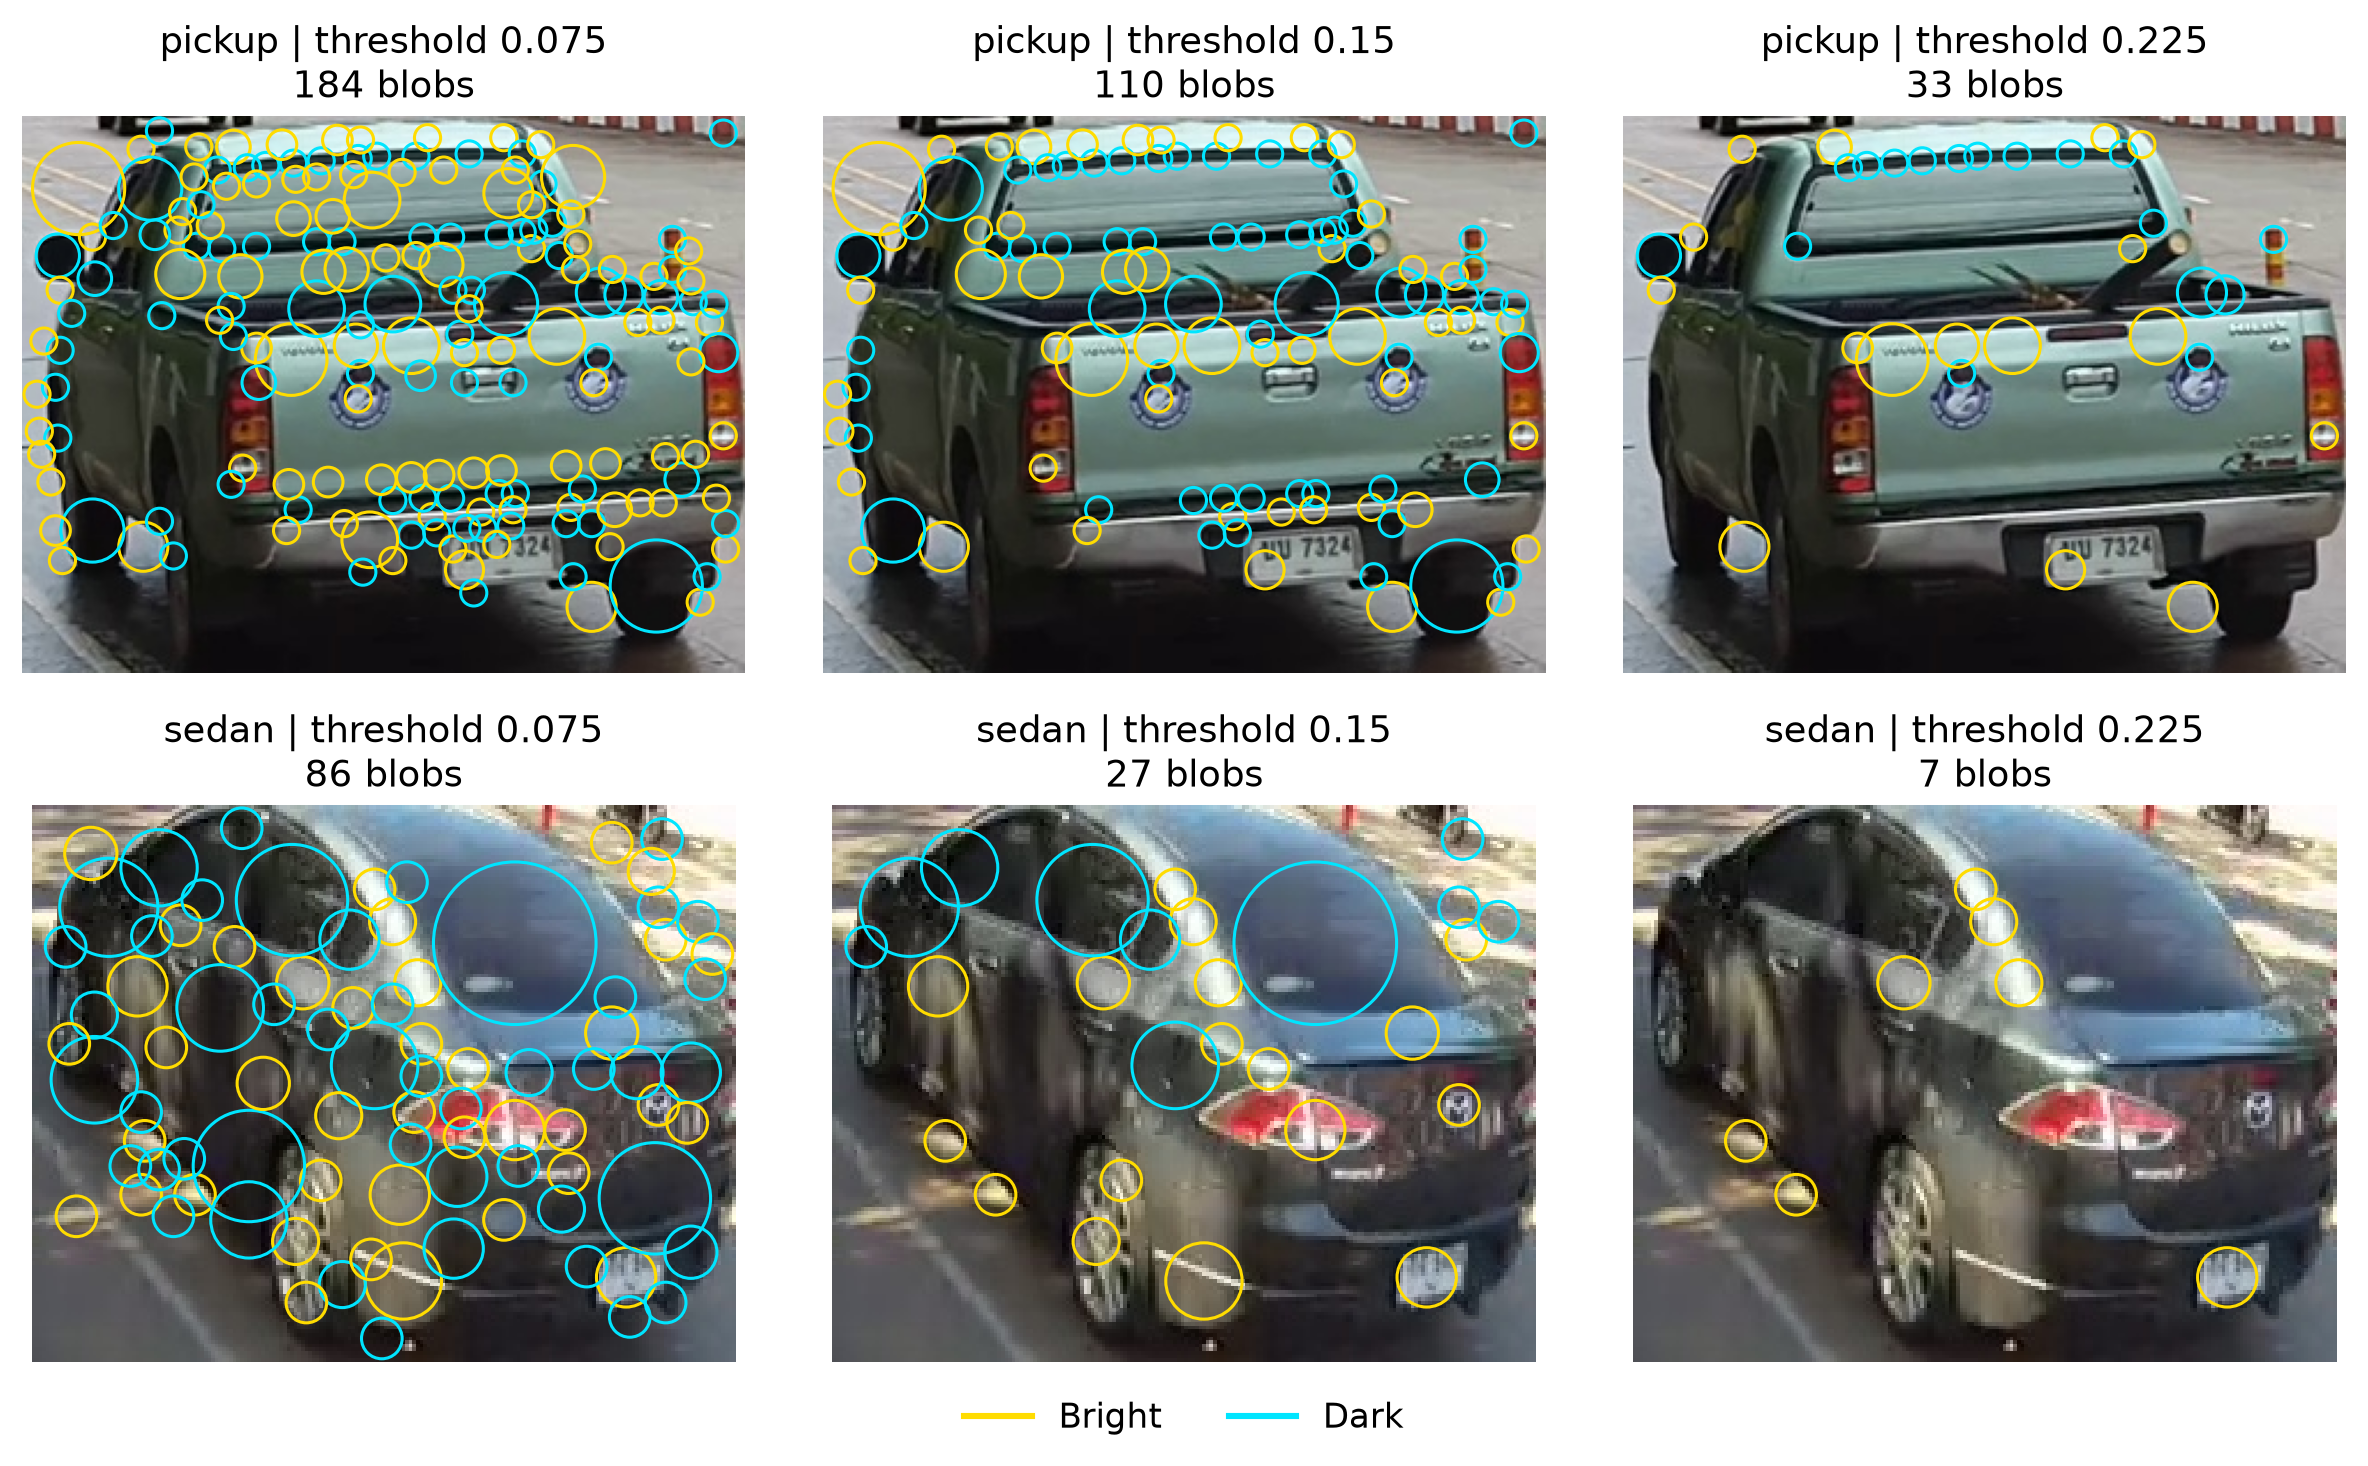
\includegraphics[width=\linewidth]{Images/blob_report_thresholds.png}
 \caption{Threshold sensitivity for pickup (top) and sedan (bottom).
 Threshold increases from left to right; every other parameter remains at
 baseline. Panel counts concern the individual example images.}
 \label{fig:blob-parameters}
\end{figure}

The pickup counts fall from 184 to 110 to 33, while the sedan counts fall from
86 to 27 to 7. At the high threshold, repeated pickup window-edge responses
remain, but the broad dark sedan window response disappears and several bright
reflections remain. A large blob therefore need not have a strong response.
The rise in dataset-wide mean radius is a distributional result, not a rule
for each feature, and fewer detections do not establish better detection.

\textbf{Scale range.} Raising the minimum scale to 7 excludes radii below
9.90 pixels, reducing the total to 35,726 and increasing mean radius to 11.93
pixels. Increasing the maximum scale to 30 permits radii up to 42.43 pixels,
but gives a slightly lower count than baseline (84,213). Because the number
of scales remains 12, changing either endpoint also changes the intermediate
sampling grid. The result therefore combines a changed size range with changed
scale sampling; overlap suppression and frame exclusion further affect which
candidates survive.

\textbf{Overlap and pre-smoothing.} Reducing the overlap limit from 0.5 to 0.2
leaves 77,302 blobs by rejecting more competing circles, potentially including
nearby distinct features. Additional smoothing with $\sigma_{\mathrm{pre}}=2$
leaves 44,825 blobs with a mean radius of 9.42 pixels. This reduction in count
and increase in mean radius are consistent with suppression of fine detail.

The parameters control different aspects of the representation: threshold
selects response strength, scale limits select feature size, and overlap
suppression removes competing detections. Their suitability therefore depends
on the intended feature, such as a compact reflection or a broader dark region.
The experiments establish sensitivity to these choices; without a defined
target and independent annotations, they do not establish an optimal setting.
\FloatBarrier
